%=========PROBLEM 1============================================
\section*{Problem 1}

This problem wants us to learn how to plot a function and making it legible when it needs to be included in \LaTeX documents such as this homework. 

\begin{figure}[t]
    \centering
    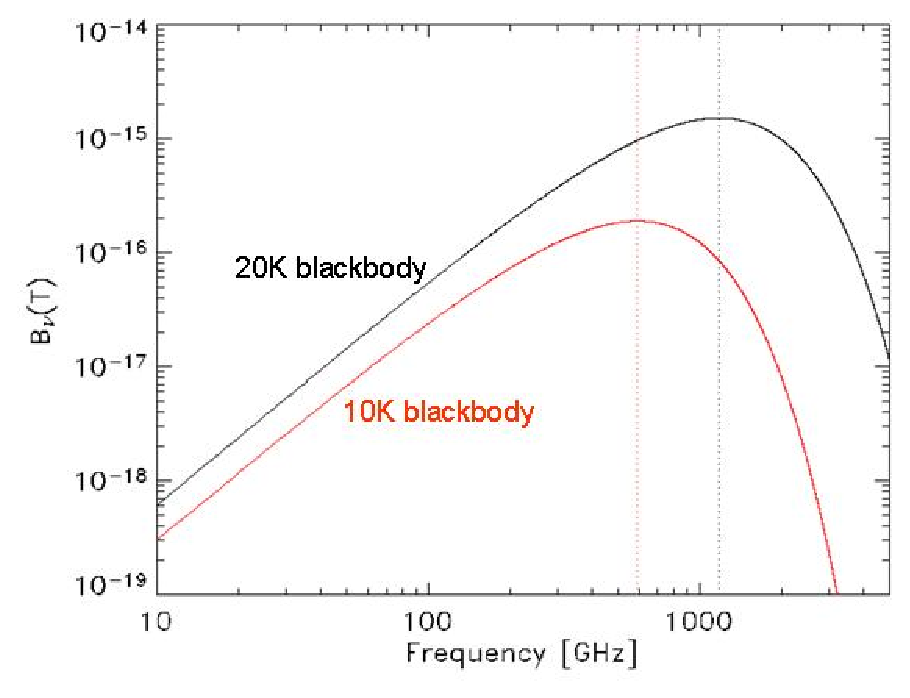
\includegraphics[scale=1]{figures/planck.eps}
    \caption{Original Plot}
    \label{fig:grantOriginalPlot}
\end{figure}

\begin{figure}[t]
    \centering
    \includegraphics[scale=1]{figures/hw01prob1-1.png}
    \caption{Plot created by python code "hw01prob1-1.py"}
    \label{fig:blackbodyRadiationPlot}
\end{figure}

The requirements are:

\begin{itemize}
    \item Axis labels should be readable and correct
    \item Text in plot should be the same size as text in document. \textit{(optional but recommended)}
    \item Plot should accurately show the blackbody radiation of two blackbodies, \SI{10}{\kelvin} and \SI{20}{\kelvin}.
\end{itemize}

The steps followed to recreate this plot were the following:
\begin{enumerate}
    \item \textbf{Look up the constants.}
    
     I look up the current constants on the NIST website which were defined on the 2018 CODATA. To make it easier for the future me, I define a function with my constants which can be updated as needed.
     
    \item \textbf{Determined my variables.}
    
    \item \textbf{Calculate the blackbody radiation and frequency of the peak.}
    
    To calculate the blackbody radiation I used Planck's Law given by,
        \begin{equation}
        B_\nu(T) = \frac{2h\nu^3}{c^2}\frac{1}{e^{h\nu /kT}-1} \mbox{ [Hz]}
        \label{eq:Plancks}
        \end{equation}
    To calculate the maximum frequency I used Wien's Displacement Law given by,
        \begin{equation}
         \nu_{\rm{max}} = 5.879\times 10^{10} T \mbox{ [\si{\hertz}]}
        \label{eq:WienDisp}
        \end{equation}. 
    In the code, these equations are defined as functions.
    
    \item \textbf{Plot my equations.}
    
    To show the blackbody radiation correctly, both the frequency axis and the radiation axis need to be in log form. To do this, I use the loglog command. 
    The maximum frequency is shown as a vertical line, so to achieve this a I use the axvline command.
    
    \item \textbf{Customize the plot to achieve a readable plot.}
    
    To customize the plot I define the following main parameters:
        \begin{itemize}
            \item Font: 8pt
            \item Width: 3.39 for it to show in a single column size or 6.9 for use a double column size. 
            \item Height: 2.41 for a single column or 4.26 for a double column. The height was calculate from the Golden Mean $= \sqrt{5}-1 / 2 $, which is determined to be an aesthetic ratio. 
        \end{itemize}
\end{enumerate}

The final figure produced is shown on Figure  \ref{fig:blackbodyRadiationPlot}.